% se puede agregar la opción [english] para 
%  memorias o tesis en inglés (borrando el archivo .aux)
\documentclass{umemoria} 

\depto{Departamento de las ciencias de computación}
\author{Nombre Completo Autor}
\title{Implementación de un servidor de nombres usando la librería dns-rust}


\memoria{Ingeniero Civil en Computación}
%\tesis{Doctor en ???} % incluir solo este comando para doctorados

% puede haber varios profesores guía seperados por coma;
% pero si es una memoria, solo puede haber un profesor guía
\guia{Javier Bustos} 

% puede haber varios profesores co-guía seperados por coma;
% pero si es una memoria, el profesor co-guía será el primer
% integrante de la comisión
%\coguia{Nombre Completo Co-Guía} % incluir en caso de co-guía de *tesis*

%\cotutela{Nombre Institución} % incluir en caso de cotutela

\comision{Nombre Completo Uno,Nombre Completo Dos,Nombre Completo Tres}

%\auspicio{Nombre Institución} % incluir en caso de recibir financiamiento

% tiene que ser el año en que se da el examen de título/grado (defensa)
%\anho{2021} % incluir solo para reemplazar el año actual

\usepackage{lipsum}
\usepackage[fixlanguage]{babelbib}
\usepackage{url}
\usepackage{listings}
\usepackage{xcolor}

\usepackage{array}
\usepackage{geometry}
\usepackage{longtable}
\usepackage{multicol}
\usepackage{amsmath}
\usepackage{caption}
\usepackage{fancyhdr}
\usepackage{graphicx}

\usepackage{listings}
\usepackage{xcolor}

\usepackage{tikz}
\usetikzlibrary{shapes.geometric, arrows.meta, positioning}
\tikzstyle{startstop} = [rectangle, rounded corners, minimum width=3cm, minimum height=1cm, text centered, draw=black, fill=red!30]
\tikzstyle{process} = [rectangle, minimum width=3.5cm, minimum height=1cm, text centered, draw=black, fill=blue!15]
\tikzstyle{decision} = [diamond, aspect=2, text centered, draw=black, fill=green!25]
\tikzstyle{arrow} = [thick,->,>=stealth]

\lstdefinelanguage{Rust}{
  keywords=[1]{pub, struct, fn, let, mut, match, impl, for, in, loop, while, if, else, use, mod, crate, ref, return, break, continue, as, const},
  keywords=[2]{String, HashMap, usize, Result, Option},
  keywordstyle=[1]\color{blue}\bfseries,
  keywordstyle=[2]\color{teal},
  identifierstyle=\ttfamily,
  comment=[l]{//},
  commentstyle=\color{gray}\ttfamily,
  stringstyle=\color{orange},
  morestring=[b]",
  morecomment=[s]{/*}{*/},
  sensitive=true
}

\lstset{
  language=Rust,
  basicstyle=\ttfamily\small,
  numbers=left,
  numberstyle=\tiny\color{gray},
  stepnumber=1,
  numbersep=5pt,
  tabsize=2,
  showspaces=false,
  showstringspaces=false,
  frame=single,
  breaklines=true,
  captionpos=b
}


% Define custom colors
\definecolor{codegreen}{rgb}{0,0.6,0}
\definecolor{codegray}{rgb}{0.5,0.5,0.5}
\definecolor{codepurple}{rgb}{0.58,0,0.82}
\definecolor{backcolour}{rgb}{0.95,0.95,0.92}

% Custom style for code
\lstdefinestyle{mystyle}{
    backgroundcolor=\color{backcolour},   
    commentstyle=\color{codegreen},
    keywordstyle=\color{purple},
    numberstyle=\tiny\color{codegray},
    stringstyle=\color{codepurple},
    basicstyle=\ttfamily\footnotesize,
    breakatwhitespace=false,         
    breaklines=true,                 
    captionpos=b,                    
    keepspaces=true,                 
    numbers=left,                    
    numbersep=5pt,                  
    showspaces=false,                
    showstringspaces=false,
    showtabs=false,                  
    tabsize=2
}
\lstset{style=mystyle}

\begin{document}

\frontmatter
\maketitle

\begin{resumen}
\lipsum[1-4]
\end{resumen}

% opcional: incluir para tesis en inglés;
%  en este caso hay que tener el resumen y abstract
%   en ambos idiomas
%\begin{abstract}
%\lipsum[1-4]
%\end{abstract}

\begin{dedicatoria}
Una dedicatoria corta.
\end{dedicatoria}

\begin{thanks}
\lipsum[1-2]
\end{thanks}

\tableofcontents
\listoftables % opcional
\listoffigures % opcional

\mainmatter

\chapter{Introducción}

\section{Contexto}

DNS (Domain Name System) es un protocolo fundamental para el funcionamiento de la capa siete del modelo OSI, permitiendo que un usuario pueda 
acceder a una IP global a través de un nombre de dominio, como por ejemplo dcc.uchile.cl. Para lograr esto existen 2 actores principales: 
el Resolver y el Name Server.

El Resolver es el programa encargado de tomar una consulta de un nombre de dominio desde un dispositivo como un computador o un celular y 
transformarlo en una consulta DNS, la cual es un mensaje en bytes con una estructura definida por el protocolo DNS, con las siguientes 5 
secciones: Header, Question, Answer, Authority y Additional

El Name Server es el que conoce las IP de los dominios y es el encargado de responder las consultas DNS que envía el Resolver, pero este proceso
no es sencillo y requiere del arduo estudio y programación de los RFC (Request For Comments), documentos estandarizados de cómo debe funcionar 
el internet.

En este contexto, el área de investigación de NIC Chile (NIC Labs) implementó una librería de funciones para DNS en lenguaje Rust, como 
caso de prueba de dicha librería desean implementar un servidor de nombres (Name Server) DNS que utilicen para su propia zona niclabs.cl. 
Una zona es un conjunto de nombres de dominios hijos de un dominio padre, en este caso el dominio padre es niclabs.cl (la zona misma) y un dominio hijo podría ser a.niclabs.cl

La librería DNS-RUST  de NIC Labs sigue cabalmente las indicaciones de los RFC sin implementar ningún tipo de optimización que no sea 
referenciada por ellos, por lo que es importante la implementación del Name Server bajo esas especificaciones ya que puede ser utilizado 
más adelante para investigación y desarrollo.

Mencionar que la librería DNS-RUST es solo una herramienta que contiene las funciones necesarias para transformar un mensaje DNS en bytes a 
una estructura en Rust (parse), un Cliente y un Stub-Resolver, es decir, no posee nada relacionado a un Name Server. De esta manera todas las 
funcionalidades, estructuras de datos y algoritmos serán implementados desde cero. 

Como se verá más adelante, implementar un Name Server con todas sus funcionalidades incluyendo las que aún no posee la librería es un trabajo 
que toma más de un semestre, de hecho, para tener más contexto, el Stub-Resolver de la libería DNS-RUST fue desarrollado por años de manera 
grupal, por lo que es lógico pensar que su contraparte (un Name Server) no puede ser completado al 100 porciento por una sola persona en un 
semestre, provocando así que el trabajo a realizar sea acotado sólo a las funcionalidades de DNS Security Extension, Extension DNS 0, 
creación de estructuras de datos basadas en el \texttt{masterfile}, implementación del algoritmo de búsqueda del Name Server y conexiones UDP-TCP 
asíncrónicas.



\section{Glosario}
Antes de seguir con el desarrollo de este informe, es necesario abarcar ciertos conceptos específicos que se referenciarán más adelante:

\begin{itemize}
    \item Stub-Resolver: Es un resolver que utiliza un resolver recursivo, el cual se encarga de todo el proceso real para responder a una 
    consulta DNS. Estos resolvers recursivos son complejos y un stub-resolver suele utilizar los creados por Google y otras grandes empresas.
    \item Extension DNS 0 (EDNS0): Primera extensión del protocolo DNS, incluyendo la capacidad de aumentar el tamaño de los mensajes DNS 
    (consultas y responses).
    \item DNS Security Extension (DNSSEC): Extensión de seguridad del protocolo DNS, permitiendo mensajes firmados y validaciones basadas 
    en criptografia.
    \item Resource Record (RR): Estructura de datos que se envía como respuesta desde el Name Server. Existen muchos tipos, cada uno con 
    sus especificaciones.
    \item RRset: Conjunto de RR's que poseen el mismo nombre de dominio, tipo y clase.
    \item Catalogo: Estructura jerárquica con las zonas que maneja el Name Server.
    \item Arbol de dominios: Estructura jerárquica que contiene los RRSets de los dominios guardados por el Name Server.
    \item Tipos de Resource Records clasicos:
        \begin{itemize}
            \item Answer (A): Dirección IP del nombre de dominio solicitado.
            \item Name Server (NS): Nombre de dominio del Name Server autoritativo que sabe responder a la consulta solicitada. 
            \item Canonical Name (CNAME): Nombre de dominio secundario-canónico que pueda tener el nombre de dominio solicitado.
            \item Optional (OPT): RR especial para Extension DNS 0 con muchas funcionalidades, pero la más importante es la de aumentar el 
            tamaño default de las consultas DNS (512 bytes).
        \end{itemize}
    \item Tipos de Resource Records de DNSSEC:
            \begin{itemize}
            \item DNS Public Key Record (DNSKEY): Contiene la llave pública necesaria para validar la firma contenida en el RRSIG.
            \item  Resource Record Signature (RRSSIG): Firma criptográfica creada a partir de una llave privada alojada en el Name Server.
            \item Delegation Signer (DS): Hash de la llave pública alojada en el Name Server padre necesario para validar el DNSKEY RR.
            \item Next Secure Record (NSEC): RR que contiene el siguiente nombre de dominio en un orden canonico dentro del arbol de dominios (
                ordenado en bytes).
        \end{itemize}
    \item Clase en un RR: Valor que determina el medio a usar en el protocolo, normalmente es de tipo $IN$ (Internet), pero también existen 
    otros tipos secundarios que no es necesario mencionar.
    \item RDATA (Response Data): Valores de retorno que contienen la información clave de un RR. Es diferente para cada tipo de RR.
\end{itemize}

\section{Objetivos}

\subsection*{Objetivo General}

El objetivo de este trabajo es construir un MVP (Producto Mínimo Viable) de un Name Server Autoritativo Iterativo capaz de controlar la zona de 
dominio del laboratorio de manera segura, eficiente, siguiendo al pie de la letra los RFC y usando las herramientas de la librería DNS-RUST como 
apoyo.

Que el Name Server sea Iterativo consiste en que su algoritmo busca el nombre de dominio solicitado dentro de su estructura de datos, si no 
tiene la respuesta directa, envía una referencia hacia otro Name Server que si podría tenerla, y si no encuentra ninguna respuesta envía un 
error. La alternativa es un Name Server recursivo que, si no conoce la respuesta a la consulta, utiliza un Resolver interno para averiguarla y 
responder, y que por su diseño y construcción no es parte de este trabajo de título.

\subsection*{Objetivos Específicos}\label{sec:obj-e}

\begin{enumerate}
\item Establecer canales de trasmisión confiables, en los protocolos de UDP y TCP asincrónicos.
\item Responder correctamente a consultas DNS de tipo basico (A, NS, CN) con sus Resource Records correspondientes.
\item Seguir estrictamente lo establecido por los RFC antiguios y actuales.
\item Asegurar seguridad con DNSSEC (DNS Security Extension), usando algoritmos de encriptación, llaves publicas y privadas, firmas y una cadena de autentificación.
\item Crear de estructuras de datos jerárquicas (árboles) a partir de un \texttt{masterfile} .
\item Conectar las herramientas de la libería DNS-RUST usando su stub-resolver como cliente y sus parses de mensajes para manejar las consultas DNS .
\item Cumplir con estándares de documentación en el código.
\item Incluir EDNS0 (Extension DNS 0) necesaria para cumplir DNSSEC. Especificamente sabiendo leer y procesar consultas del tipo OPT.


\end{enumerate}



\chapter{Marco teórico}

\section{RFC's}

Parte fundamental del protocolo DNS son los RFC, ya que definen las reglas y el comportamiento que debe seguir todo el internet
en general, y en especifico el protocolo DNS. A continuación se detallan los RFC más importantes para el desarrollo de 
este proyecto:

\subsection{RFC 1034}

\begin{itemize}
    \item Estructura de una consulta DNS, en especifico, el formato de la sección Header.
    \item Resource Records, explica campos como el owner name, tipo, clase, TTL (Time To Live) y RDATA (Response Data)
    \item Algoritmo de búsqueda de un Name Server para un nombre de dominio.
    \item Algoritmo de consulta de un Resolver.
    \item WildCards, nombres de dominios especiales que permiten que subdominios no definidos respondan con la misma información.
\end{itemize}

\subsection{RFC 1035}

\begin{itemize}
    \item Significado de los valores y flags dentro del Header.
    \item Formatos de los RDATA de tipos comunes de RR (A, SOA, NS, CNAME).
    \item Conexiones UDP y TCP y sus usos en cada caso.
    \item \texttt{masterfiles} y como a partir de estos crear las estructuras de datos.
    \item Arquitectura del Name Server, específicamente el uso de la concurrencia-asincronismo en el procesamiento de consultas.
\end{itemize}


\subsection{RFC 4033}
\begin{itemize}
    \item Glosario de conceptos DNSKEY: Cadena de autentificación, pares de llaves criptogracias, puntos de delegación, etc.
    \item Dos nuevos bits en el Header: Checking Disabled (CD) y Authenticated Data (AD).
    \item Uso de EDNS0 para aumentar el tamaño base (512 bytes) de una consulta DNS. Esto ya que las llaves y firmas usadas en DNSSEC suelen ser de gran tamaño.
\end{itemize}

\subsection{RFC 4034}
\begin{itemize}
    \item Formatos de los RDATA de los tipos de DNSSEC (DNSKEY, RRSIG, DS y NSEC)
    \item Forma Canonica para ordenar los RRSets y los nombres de dominios.
    \item Algoritmos de encriptación
    \item Algoritmo para calcular el Key Tag del RRset de DNSKEY
\end{itemize}

\section{Estado del Arte}
En el contexto actual existen distintos software para crear un Name Server, algunos comerciales como Bind9~\cite{Bind9} que está escrito en C y que es Open Source y otros como PowerDNS~\cite{PowerDNS} que es de código privado. Estas son herramientas útiles, pero no es posible verificar si cumplen estrictamente con las especificaciones de los RFC, lo que resulta especialmente importante para NIC Labs. Además, estos programas no están escritos en Rust, lenguaje de programación muy valorado por su alto nivel de seguridad en accesos a memoria~\cite{SafeRust}.

Es importante tener seguridad en el acceso a memoria, ya que previamente se han encontrado o aprovechado vulnerabilidades de Name Servers escritos en otros lenguajes. A continuación se verán algunos ejemplos:

\subsection{ISC BIND server heap overflow de 4 bytes}
Como se vio previamente Bind9 es uno de los software más usados para crear Name Servers, pero a pesar de esto en febrero de 2021 se reportó y se parchó una vulnerabilidad que se mantuvo por 15 años sin ser explotada, y que fue descubierta por un investigador anónimo ~\cite{VulnerabilidadBind}.

La vulnerabilidad permite de manera remota y sin autentificación envenenar el caché del server (Poisoned Cache Attack), provocando así que el caché guarde y responda IPs a sitios inseguros a consultas legítimas, afectando gravemente a todos los usuarios que consulten a este Name Server.


La vulnerabilidad nace por el siguiente código escrito en C:
\begin{lstlisting}[language=C]
static int 
der_get_oid(const unsigned char *p, size_t len, oid *data, size_t *size) { 
// ... 
data->components = malloc(len * sizeof(*data->components));   // <-- (1) 
    if (data->components == NULL) { 
      return (ENOMEM); 
    } 
    data->components[0] = (*p) / 40;    // <-- (2) 
    data->components[1] = (*p) % 40; 
    --len;               // <-- (3) 
    ++p; 
    for (n = 2; len > 0U; ++n) { 
        unsigned u = 0; 
 
        do { 
            --len; 
            u = u * 128 + (*p++ % 128); 
        } while (len > 0U && p[-1] & 0x80); 
        data->components[n] = u;      // <-- (4) 
    } 
// ... 
}
\end{lstlisting}

La función provoca un overflow de 4 bytes al final del arreglo, permitiendo al atacante utilizar esos 4 bytes para inyectar código malicioso y 
provocar el envenenamiento del caché.

Con el lenguaje Rust habría sido más difícil que ocurriera, ya que el compilador hubiese prevenido al programador al momento de asignar un valor 
fuera de los límites del vector original.

\subsection{Vulnerabilidades en Dnsmasq}

Dnsmasq ~\cite{Dnsmasq} es un redireccionador de DNS usado por servidores que en primera instancia no quieren usar la red global de Name Servers 
y utilizar únicamente el caché proporcionado por este servicio. En general se usa para sistemas embebidos con zonas muy pequeñas que no necesitan
 mucha comunicación con otros servidores.

El problema con este software escrito en el lenguaje C es que presentó múltiples vulnerabilidades simultáneamente, en concreto se encontraron 4 
vulnerabilidades de buffer overflow (provocadas por errores directos en el código) y 3 vulnerabilidades de validación que podrían provocar 
envenenamiento del caché, a continuación se muestran las últimas 3 vulnerabilidades:

\begin{itemize}
\item CVE-2020-25681: No se validaba el par (dirección, puerto) ni el ID de la consulta DNS al recibirlas.
\item CVE-2020-25685: Usaba un algoritmo de hashing débil (CRC32), vulnerable a ataques.
\item CVE-2020-25686: Dnsmasq no chequeaba que una consulta hubiese terminado de procesarse para recibir y redireccionar otra igual 
(con el mismo nombre de dominio, tipo y clase), por lo que el atacante puede enviar muchas consultas equivalentes tratando de adivinar el ID 
para que así el cliente la acepte como válida, y esto no es tan improbable por la paradoja del cumpleaños ~\cite{BirthdayAttacks}
\end{itemize}


A pesar de que estas 3 vulnerabilidades mencionadas no sean consecuencia directa del lenguaje usado, sino de la mala verificación y uso de 
algoritmos, es fundamental conocerlas y analizarlas para evitar repetir errores ya cometidos.

\subsection{Por qué seguir los RFC}

Los RFC son los documentos estandarizados que explican cómo debe ser implementado el internet en sus diferentes capas, pero, 
¿Qué consecuencias puede tener ignorar las reglas de estos documentos?

A continuación se verán vulnerabilidades descubiertas en Name Servers que no siguieron indicaciones \textbf{obligatorias} dadas por los RFC.

\subsubsection{Falta de validaciones en los nombres de dominio}

Según el RFC 1035 ~\cite{RFC1035} los nombres de dominio deben seguir un estándar y cumplir ciertas reglas, en específico deben cumplir lo siguiente:

\begin{itemize}
\item Tener un largo de máximo 255 bytes en total.
\item Cada label dentro del nombre de dominio puede tener un máximo de 63 bytes.
\item Terminar con un carácter \textbackslash 0.
\end{itemize}

Todas esas condiciones deben ser verificadas, de lo contrario pueden ocurrir diversos ataques de buffer overflow, ataques de Denegación de 
Servicio (DDoS) y ejecución de código remoto ~\cite{AtaquesRFC}.

En concreto se descubrió una vulnerabilidad ~\cite{Ethernut} consecuencia de la falta de validación del largo de un nombre de dominio dentro de l
a implementación de DNS en Nut/OS en un dispositivo Ethernut (dispositivo de IoT). Solamente con esta falla se podría ejecutar código remoto y/o 
un ataque DDoS.

De manera similar, se encontraron muchas vulnerabilidades en dispositivos IoT causadas por la falta de validación del largo de los labels del 
nombre de dominio ~\cite{LabelsIOT}.

\subsection{Otras implementaciones de Name Servers en Rust}

Existen otras librerías de DNS (en específico con el módulo de Name Server) que están siendo desarrolladas por otras organizaciones, como 
HickoryDNS \cite{HickoryDNS} y domain\cite{NLnetLabs} de NLnetLabs. Estas librerías están en un punto muy alto de desarrollo, pero es 
importante conocer y comprender cuáles han sido sus errores. A continuación se verán algunos ejemplos:

\subsubsection{Hickory vulnerabilidad DNSSEC por verificación de un solo DNSKEY}

En el Resolver de Hickory al momento de validar un DNSKEY a través del ancla de confianza (trust anchor), que es un registro ya guardado en el 
Resolver para terminar la cadena de autenticación, si el DNSKEY es validado, por error se valida cualquier otro DNSKEY proveniente del mismo 
RRSet~\cite{HickoryBug}, lo cual es incorrecto, ya que cada uno de estos debe ser validado de forma individual.



\subsubsection{Error al firmar la zona debido a glue records}

Para firmar una zona (aplicando DNSSEC) se necesita encontrar el SOA RR, el cual permite verificar que la zona es legítima, y este RR siempre 
debe estar en el Apex Zone (en la zona más alta de la estructura de datos jerárquica), pero si hay algún glue RR 
(los cuales tienen las IP de otros Name Servers) estos pueden anteceder al SOA debido al ordenamiento canónico (por bytes).

Este reordenamiento provocaba que el proceso de firma no encontrara el SOA RR y por lo tanto no firmara una zona válida ~\cite{NLnetLabsBug}.







\chapter{Conneciones UDP y TCP}

El servidor DNS implementado usa la librería \texttt{tokio} para atender consultas en UDP y TCP de forma asíncrona y concurrente. 
Además de la funcionalidad básica de recibir y devolver respuestas, también soporta EDNS0, detecta y respeta el payload máximo 
anunciado por el cliente en el registro OPT, maneja el estándar DNSSEC (lectura del bit DO) y protege operaciones críticas
con timeouts para evitar bloqueos y bucles infinitos. También se manejan correctamente errores de parseo (se responde FORMERR) y
se implementa el comportamiento para truncamiento (TC) sobre UDP con fallback a TCP.

A continuación se describen las implementaciones específicas para cada protocolo.

\section{UDP}

El servidor UDP está implementado en la estructura \texttt{ServerUDPConnection}, que contiene los siguientes campos y métodos:

\begin{table}[h!]
\centering
\renewcommand{\arraystretch}{1,1}

\begin{tabular}{|p{0.95\linewidth}|}
\hline
\multicolumn{1}{|c|}{\textbf{ServerUDPConnection}} \\
\hline
\textbf{Campos} \\
\hline
\texttt{- timeout: tokio::time::Duration} \\
\texttt{- payload\_size: usize} \\
\hline
\textbf{Métodos Públicos} \\
\hline
\texttt{+ new\_udp(timeout: Duration, payload\_size: usize) -> Self} \\
\texttt{+ new\_default(timeout: Duration) -> Self} \\
\texttt{+ receive\_and\_response(\&mut self) -> Result<(), ServerError>} \\
\hline
\textbf{Métodos Privados / Auxiliares} \\
\hline
\texttt{- handle\_dns\_message\_udp\_with\_timeout (} \\
\texttt{\ \ timeout\_server: Duration, recv\_buf: \&[u8],} \\
\texttt{\ \ socket: \&UdpSocket, client\_addr: SocketAddr,} \\
\texttt{\ \ tc\_case: bool, len: usize ) ->  Result<(), ServerError>} \\
\hline
\end{tabular}
\end{table}

%%Explicacion de los campos

El campo \texttt{timeout} define el tiempo máximo que el servidor esperará para recibir una consulta o enviar una respuesta antes de abortar la operación.
El campo \texttt{payload\_size} establece el tamaño máximo de la consulta DNS que el servidor puede procesar.

%%Explicacion de los metodos

Los métodos definidos incluyen funciones típicas como \texttt{new} y \texttt{new\_default}, que permiten crear 
una instancia de la clase con parámetros personalizados o por defecto. Sin embargo, la función más relevante es \texttt{receive\_and\_response}, 
la cual se encarga de recibir y responder de manera asíncrona a las consultas DNS enviadas por los clientes.

%%Explicación del flujo

La funcion \texttt{receive\_and\_response} sigue los siguientes pasos:
\begin{itemize}
    \item Crea un socket UDP y se enlaza a localhost en el puerto 53.
    \item Entra en un bucle infinito donde se espera recibir consultas DNS.
    \item Crean los distintos threads con \texttt{tokio} para manejar la concurrencia.
    \item En cada thread, si el tamaño de la consulta es mayor al \texttt{payload\_size}, se usa la función \texttt{handle\_dns\_message\_udp\_with\_timeout}
          con \texttt{tc\_case} en true, de lo contrario se llama a la misma función con \texttt{tc\_case} en false.
\end{itemize}

%Imagen del diagrama de flujo desde la carpeta diagramas, con 

\begin{figure}[h!]
    \centering
    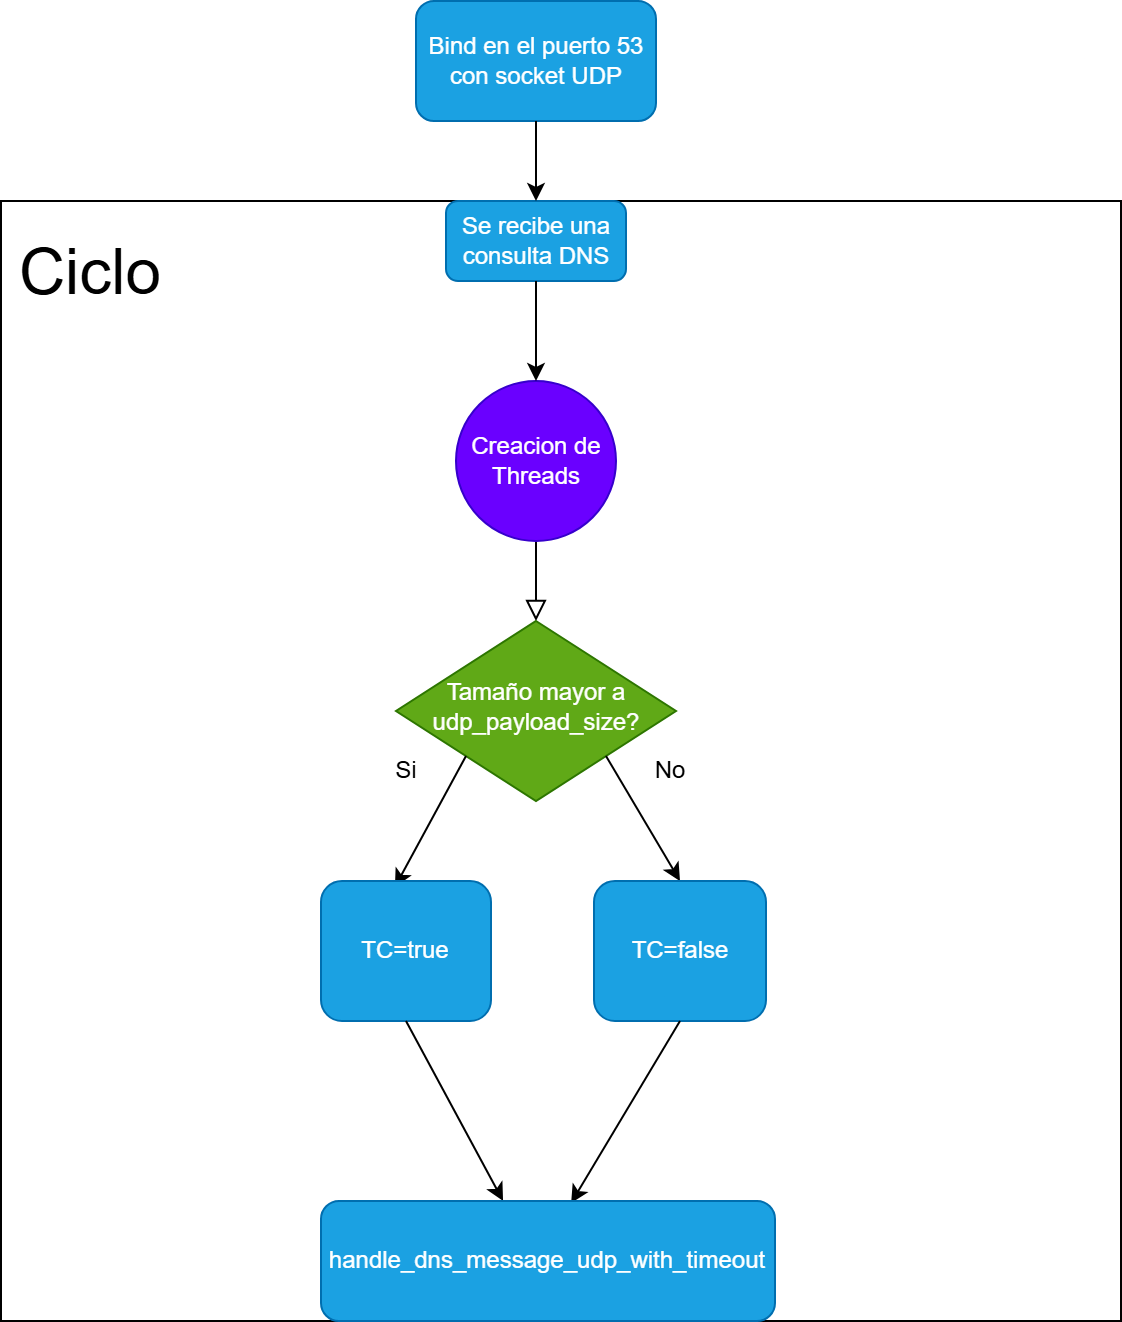
\includegraphics[width=0.7\textwidth]{diagramas/recieve_and_response.png}
    \label{fig:udp_flowchart}
\end{figure}


Con respecto a la función auxiliar \texttt{handle\_dns\_message\_udp\_with\_timeout}, esta se encarga de:

\begin{itemize}
    \item Parsear el \textbf{header DNS} de los primeros 12 bytes del buffer recibido.  
    \item Intenta parsear el \textbf{mensaje DNS completo} (\texttt{DnsMessage::from\_bytes}) bajo un \texttt{timeout}.
    \begin{itemize}
        \item Si falla el parsing, se responde con un \texttt{RCODE=FORMERR}.
        \item Si expira el timeout, se devuelve un error de timeout.
    \end{itemize}

    \item Si \texttt{tc\_case} es verdadero:
    \begin{itemize}
        \item Se clona el mensaje original.
        \item Se activa el bit \texttt{TC} en el header de respuesta.
        \item Se reenvía el mensaje original truncado al cliente.
        \item Se termina la ejecución.
    \end{itemize}

    \item Si no es un TC case, se busca si el mensaje contiene un registro \texttt{OPT} (EDNS0):
    \begin{itemize}
        \item Si hay \texttt{OPT}, se obtiene el \textbf{DO bit} desde el campo TTL.
        \item Dependiendo del DO bit:
        \begin{itemize}
            \item Si está activo, se llama a \texttt{lookup\_data} con \texttt{dnssec=true}.
            \item Si no está activo, se llama a \texttt{lookup\_data} con \texttt{dnssec=false}.
        \end{itemize}
        \item Se serializa la respuesta.
        \item Se compara el tamaño de la respuesta con el valor de \texttt{UDP payload size} del registro OPT.
        \begin{itemize}
            \item Si la respuesta es mayor al tamaño permitido por el cliente:
            \begin{itemize}
                \item Se marca el TC bit en la cabecera original.
                \item Se responde con la versión truncada.
            \end{itemize}
            \item Si cabe dentro del tamaño permitido:
            \begin{itemize}
                \item Se envía la respuesta completa.
            \end{itemize}
        \end{itemize}
    \end{itemize}

    \item Si no hay EDNS0 (sin registro OPT):
    \begin{itemize}
        \item Se llama a \texttt{lookup\_data} con \texttt{dnssec=false}.
        \item Se envía la respuesta al cliente.
    \end{itemize}
\end{itemize}

\chapter{Estructura de Datos}
\lipsum[50-60]
\chapter{Algoritmo de Búsqueda}
\lipsum[50-60]
\chapter{EDNS0}
\lipsum[50-60]
\chapter{DNSSEC}
\lipsum[50-60]
\chapter{Discusiones}
\lipsum[50-60]
\chapter{Conclusiones}
\lipsum[50-60]


% ver https://www.overleaf.com/learn/latex/Glossaries
% \input{glosario.tex} % opcional

\nocite{*}
\bibliographystyle{plain}
\bibliography{bibliografia}

% opcional ...
\begin{appendices}
\chapter{Anexo}
\lipsum[50-60]
\end{appendices}
\end{document}